%\setcounter{chapter}{4}
\chapter{Stereo Vision}
\label{chap:stereo_vision}

\section{Introduction}

\Fig{\ref{fig:titanic}}{a} shows a {\bf stereo anaglyph}
\index{Stereo anaglyph}
of the ill-fated ocean liner, the Titanic, from \cite{McManus2022}.  This was taken with two cameras, one displaced laterally from the other.  The right camera's image appears in red in this image, and the left camera image is in cyan.  If you view this image with a red filter covering the left eye, and a cyan filter covering the right (\fig{\ref{fig:titanic}}[b]) then the right eye will see only the right camera's image (analogously for the left eye), allowing the ship to pop-out into a three-dimensional (3D) stereo image.  Note that the relative displacement between each camera's image of the smokestacks changes as a function of their depth, which allows us to form a 3D interpretation of the ship when viewing the image with the glasses (\fig{\ref{fig:titanic}}[b]).

\begin{figure}[h]
    \centerline{
        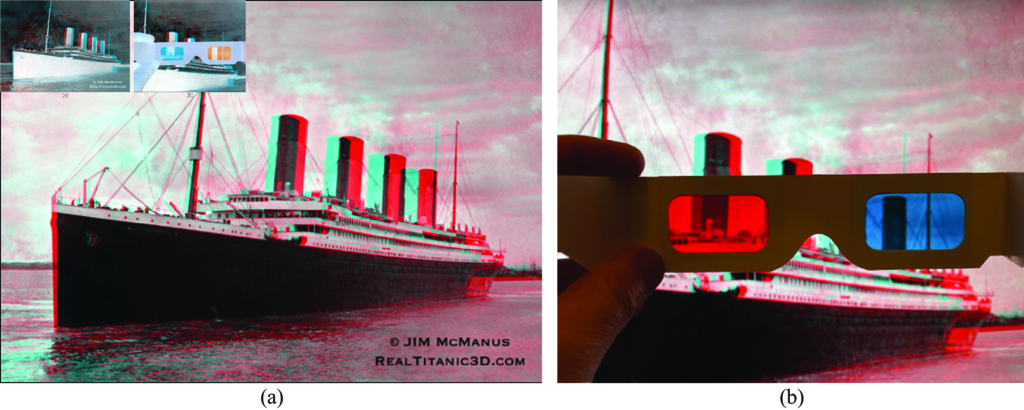
\includegraphics[width=1\linewidth]{figures/3d_scene_understanding/titanic.eps}
    }
    %\sublabel{a}{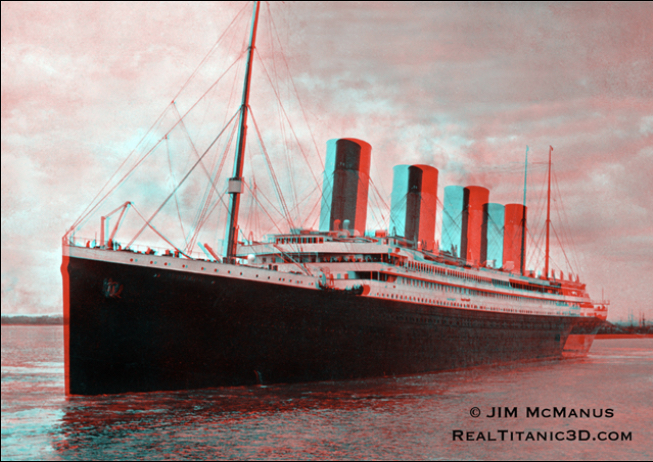
\includegraphics[width=0.5\linewidth]{figures/stereo/titanic.jpg}}
    %\sublabel{b}{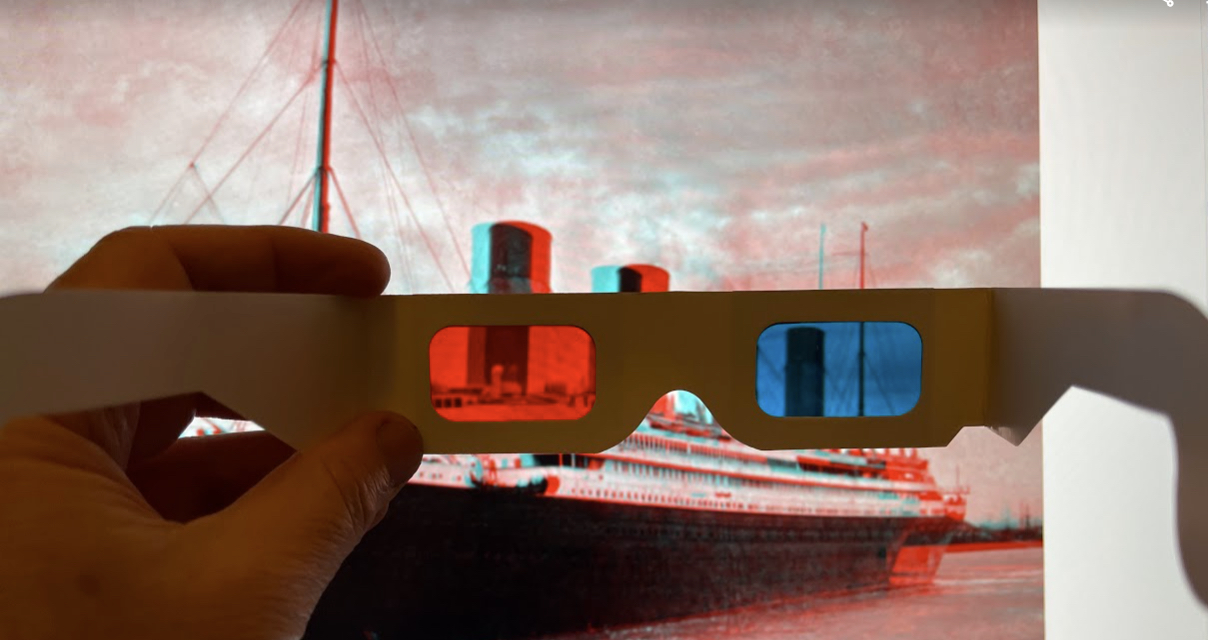
\includegraphics[width=0.5\linewidth]{figures/stereo/stereoglasses.jpg}}}
    \caption{(a) Stereo anaglyph of the Titanic \cite{McManus2022}.  The red image shows the right eye's view, and cyan the left eye's view.  (b) When viewed through red/cyan stereo glasses the cyan variations appear in the left eye and the red variations appear to the right eye, creating a perception of 3D.}
    \label{fig:titanic}
\end{figure}


In this chapter, we study how to compute depth from a pair of images from spatially offset cameras, such as those of \fig{\ref{fig:titanic}}.  There are two parts to the depth computation, usually handled separately:  (1) analyzing the geometry of the camera projections, which allows for triangulating depth once image offsets are known; and (2) calculating the offset between matching parts of the objects depicted in each image.  Different techniques are used in each part.  We first address the geometry, asking where points matching those in a first image can lie in the second image. A manipulation, called {\bf image rectification}, is often used to place the locus of potential matches along a pixel row.  Then, assuming a rectified image pair, we will address the second part of the depth computation, computing the offsets between matching image points.



\section{Stereo Cues}

How can we estimate depth from two pictures taken by two cameras placed at different locations? Let's first gain some intuition about the cues that are useful to estimate distances from two views captured at two separate observation points.

\subsection{How Far Away Is a Boat?}



To give an intuition on how depth from stereo vision works, let's first look at a simple geometry problem of practical use: How do we estimate how far away a boat is from the coast?
\marginnote{Sailors can use tricks to estimate distances using methods related to the ones presented in this chapter. These techniques can be useful when the electronics on the boat are out.}
% https://www.youtube.com/watch?v=lj19dFVlotw

We can solve this problem in several ways. We will briefly discuss two methods. The first one uses a single observation point but will use the horizon line as a reference. The second method will use two observation points. Both methods are illustrated in \fig{\ref{fig:2boats}}.


\begin{figure}[t]
    \centerline{
        \includegraphics[width=1\linewidth]{figures/3d_scene_understanding/boats.eps}
    }
    \caption{Two methods to estimate the distance of a boat from the coast. (left) The first method uses a single observation point, with knowledge of the observer's height above the water.  (right) The second method uses two observation points.}
    \label{fig:2boats}
\end{figure}

The first method measures the location of the boat relative to the horizon line. An observer is standing on top of an elevated point (a mountain, tower, or building) at a known height, $h$. The observer measures the angle $\alpha$ between the horizontal (obtained by pointing toward the horizon) and the position of the boat. We can the derive the boat distance to the base of the point of observation, $d$ by the simple trigonometric relation:
\begin{equation}
    d = \frac{h}{\tan (\alpha)}
\end{equation}
This method is not very accurate and might require high observation points, which might not be available, but it allows as to estimate the boat position with a single observation point, if the observer's height above the water is known. It also requires incorporating the earth curvature when the boat is far away.

The second method requires two different observation points along the coast separated by a distance $t$. At each point, we measure the angles, $\alpha$ and $\beta$, between the direction of the boat and the line connecting the two observation points. Then we can apply the following relation:
% https://en.wikipedia.org/wiki/Triangulation_(surveying)
\begin{equation}
    d = t \frac{\sin (\alpha) \sin (\beta)}{\sin (\alpha+\beta)}
\end{equation}
This method is called {\bf triangulation}. For it to work we need a large distance $t$ so that the angles are significantly different from $90$ degrees.


\subsection{Depth from Image Disparities}

When observing the world with two eyes we get two different views of the world (\fig{\ref{fig:titanic}}). The relative displacement of features across the two images ({\bf parallax effect})
\index{Parallax}
is related to the distance between the observer and the observed scene. Just as in the example of estimating the distance to boats in the sea, our brain uses disparities across the two eye views to measures distances to objects.


\marginnote{{\bf Free fusion} consists in making the eyes converge or diverge in order to fuse a stereogram without needing a stereoscope. Making it work requires practice. Try it in \fig{\ref{fig:random_dot_stereogram}}}
Our brain will use many different cues such as the ones presented in the previous chapter. But image disparity provides an independent additional cue. This is illustrated by the {\bf random dot stereograms}
\index{Random dot stereograms}
(\fig{\ref{fig:random_dot_stereogram}}) introduced by Bela Julesz \cite{Julez1971}. Random dot stereograms are a beautiful demonstration that humans can perceive depth using the relative displacement of features across two views even in the absence of any other depth cues. The random images contain no recognizable features and are quite different from the statistics of the natural world. But this seems not to affect our ability to compute the displacements between the two images and perceive 3D structure.

\begin{figure}
    \centerline{
        \includegraphics[width=1\linewidth]{figures/3d_scene_understanding/random_dot_stereogram.eps}
    }
    \caption{Random dot stereogram. Both images are almost identical. The difference is that there is a square in the middle that is displaced by a few pixels left-right between the two images. When each image it seen by one eye you should see a square floating in from of a flat background. You can use a stereoscope or free fusion to see it. %\reviewcomment{When I free-fuse this pair, I see an irregularly shaped hole in the center, opening to a plane behind the rest of the image, not a square floating in front of a background.}
    }
    \label{fig:random_dot_stereogram}
\end{figure}



\subsection{Building a Stereo Pinhole Camera}

Stereo cameras generally are built by having two cameras mounted on a rigid rig so that the camera parameters do not change over time.

We can also build a {\bf stereo pinhole camera}.
\index{Camera!Stereo pinhole}
As we discussed in \chap{\ref{chapter:imaging}}, a pinhole camera is formed by a dark chamber with a single hole in one extreme that lets light in. The light gets projected into the opposite wall, forming an image. One interesting aspect of pinhole cameras is that you can build different types of cameras by playing with the shape of the pinhole. So, let's make a new kind of pinhole camera! In particular, we can build a camera that produces anaglyph images, like the one in \fig{\ref{fig:titanic}}, in a single shot by making two pinholes instead of just one.

We will transform the pinhole camera into an anaglyph pinhole camera by making two holes and placing different color filters on each hole (\fig{\ref{fig:anaglyph}}). This will produce an image that will be the superposition of two images taken from slightly different viewpoints. Each image will have a different color. Then, to see the 3D image we can look at the picture by placing the same color filters in front of our eyes. In order to do this, we used color glasses with blue and red filters.

\begin{figure}
    \centerline{
        \includegraphics[width=1\linewidth]{figures/3d_scene_understanding/anaglyph_camera.png}
    }
    \caption{One way of playing with pinhole cameras is to build an anaglyph pinhole camera. The anaglyph pinhole camera captures stereo images by projecting an anaglyph image on the projection plane.}
    \label{fig:anaglyph}
\end{figure}

We used one of the anaglyph glasses to get the filters and placed them in front of the two pinholes. \Fig{\ref{fig:anaglyph}} shows two pictures of the two pinholes (\fig{\ref{fig:anaglyph}}[a]) and the filters positioned in front of each pinhole (\fig{\ref{fig:anaglyph}}[b]). \Fig{\ref{fig:anaglyph}}{d} is a resulting anaglyph image that appears on the projection plane
%(this picture was taken by placing a camera in the observation hole, \fig{\ref{fig:anaglyph}}). That image 
(\fig{\ref{fig:anaglyph}}[c]); this picture was taken by placing a camera in the observation hole seen at the right of \fig{\ref{fig:anaglyph}}{c}. \Fig{\ref{fig:anaglyph}}{d} should give you a 3D perception of the image when viewed with anaglyph glasses.

Here are experimental details for making the stereo pinhole camera. You will have to experiment with the distance between the two pinholes. We tried two distances: 3 in and 1.5 in. We found it easier to see the 3D for the 1.5 in images. Try to take good quality images. Once you have placed the color filters on each pinhole, you will need longer exposure times in order to get the same image quality than with the regular pinhole camera because the amount of light that enters the camera is smaller. If the images are too blurry, it will be hard to perceive 3D. Also, as you increase the distance between the pinholes, you will increase the range of distances that will provide 3D information because the parallax effect will increase. But if the images are too far apart, the visual system will not be able to fuse them and you will not see a 3D image when looking with the anaglyph glasses.

Let's now look into how to use two views to estimate the 3D structure of the observed scene.

\section{Model-Based Methods}

Let's now make more concrete the intuitions we have built in the previous sections.
We will start describing some model-based methods to estimate 3D from stereo images. Studying these models will help us understand the sources of 3D information, the constraints, and limitations that exist.

\subsection{Triangulation}

The task of stereo is to triangulate the depth of points in the world by comparing the images from two spatially offset cameras.\marginnote{If more than two cameras are used, the task is referred to as multiview stereo.}[-.5in]  To triangulate depth, we need to describe how image positions in the stereo pair relate to depth in the 3D world.



We will start with a very simple setting where both cameras are identical (same intrinsic parameters) and one is translated horizontally with respect to the other so that their optical axes are parallel, as shown in \fig{\ref{fig:stereo}}. We also will assume calibrated cameras.
The geometry shown in \fig{\ref{fig:stereo}} reveals the essence of depth estimation from the two cameras.
%The two cameras are identical and are oriented with their optical axes parallel with each other.  
Let's assume that there is one point, $\mathbf{P}$, in 3D space and we know the locations in which it projects on each camera, $[x_L,y_L]^\transpose$ for the left camera and $[x_R,y_R]^\transpose$ for the right camera, as shown in \fig{\ref{fig:stereo}}{a}. Because the two cameras are aligned horizontally, the $y$-coordinates for the projection in both cameras will be equal, $y_L=y_R$. Therefore, we can look at the top view of the setting as shown in \fig{\ref{fig:stereo}}{b}. We consider the depth estimate within a single image row.

\begin{figure}
    \centerline{
        \includegraphics[width=1\linewidth]{figures/3d_scene_understanding/triangularization_stereo.eps}
    }
    \caption{Simple stereo. (a) Two cameras, of identical focal length, $f$, and separated by an offset, $T$, image the point $P$ onto the two-dimensional (2D) points $[x_L,y_L]^\transpose$ and $[x_R,y_R]^\transpose$ at each camera.  (b) The similarity of the two triangles in leads to \eqn{\ref{eq:depthFromDisparity}} for the depth, $Z$, of the point $\mathbf{P}$.}
    \label{fig:stereo}
\end{figure}

The point $\mathbf{P}$, for which we want to estimate the depth, $Z$, appears in the left camera at position $x_L$ and in the right camera at position $x_R$.

\marginnote{To distinguish 2D image coordinates from 3D world coordinates, for this chapter, we will denote 2D image coordinates by lowercase letters, and 3D world coordinates by uppercase letters.}


A simple way to triangulate the depth, $Z$, of a point visible in both images is through similar triangles.  The two triangles (yellow triangle and yellow+orange triangle) shown in \fig{\ref{fig:stereo}}{b} are similar, and so the ratios of their height to base must be the same.  Thus we have:
\begin{equation}
    \frac{T+x_R-x_L}{Z-f} = \frac{T}{Z}
\end{equation}
Solving for $Z$ gives:
\begin{equation}
    Z =  \frac{fT}{x_L-x_R}
    \label{eq:depthFromDisparity}
\end{equation}
The difference in horizontal position of any given world point, $\mathbf{P}$, as seen in the left and right camera images, $x_L - x_R$, is called the {\bf disparity},
\index{Disparity}
and is {\em inversely proportional to the depth} $Z$ of the point $\mathbf{P}$ for this configuration of the two cameras--parallel orientation.  The task of inferring depth of any point in either image of a stereo pair thus reduces to measuring the disparity everywhere.

However, we are far from having solved the problem of perceiving 3D from two stereo images. One important assumption we have made is that we know the two corresponding projections of the point $\mathbf{P}$. But in reality the two images will be complex and we will not know which points in one camera correspond to the same 3D point on the other camera. This requires solving the {\bf stereo matching} problem.

\subsection{Stereo Matching}


First, let's examine the task visually.   \Fig{\ref{fig:stereomatch}} shows two images of an office, taken approximately 1 m apart.  The locations of several objects in \fig{\ref{fig:stereomatch}}{a} are shown in \fig{\ref{fig:stereomatch}}{b}, revealing some of the disparities that we seek to measure automatically.  As the reader can appreciate by comparing the stereo images by eye, one can compute the disparity by first localizing a feature point in one image and then finding the corresponding point in the other image, based on the visual similarity of the local image region.  To do this automatically is the crux of the stereo problem.




\begin{figure}[t]
    \centerline{
        \sublabel{a}{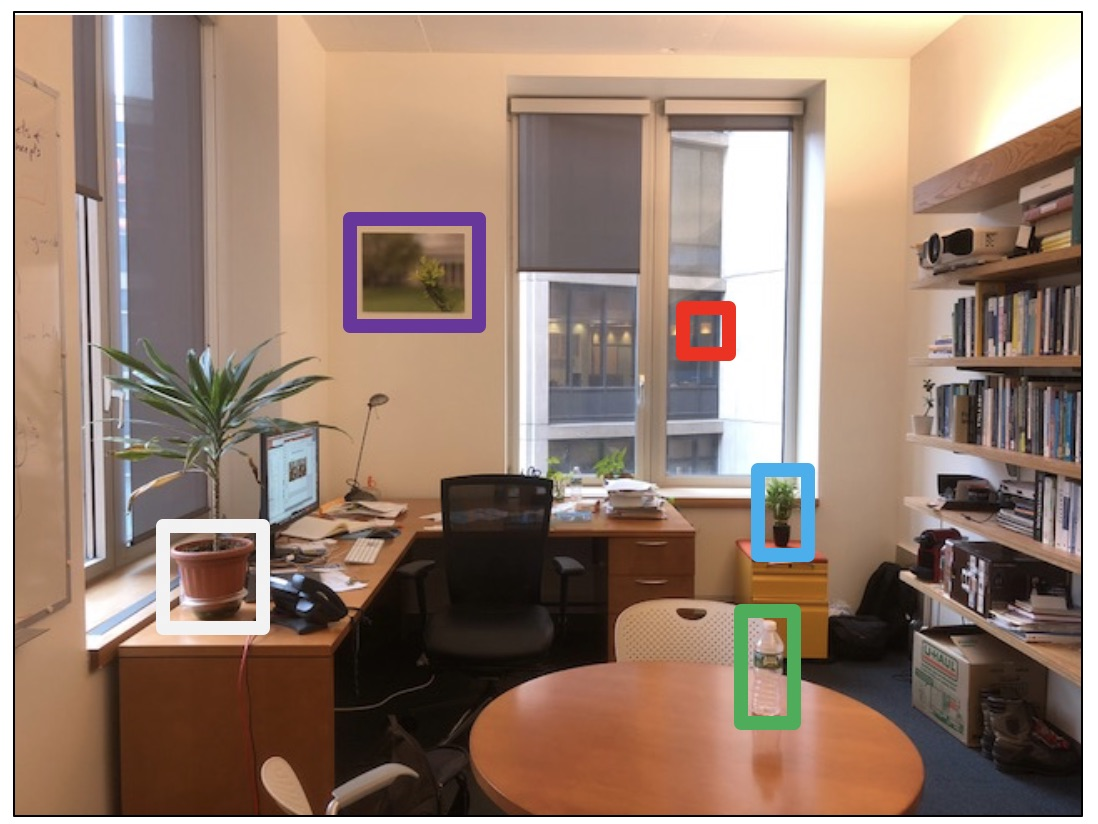
\includegraphics[width=0.475\linewidth]{figures/stereo/officeLeft.jpg}}
        \sublabel{b}{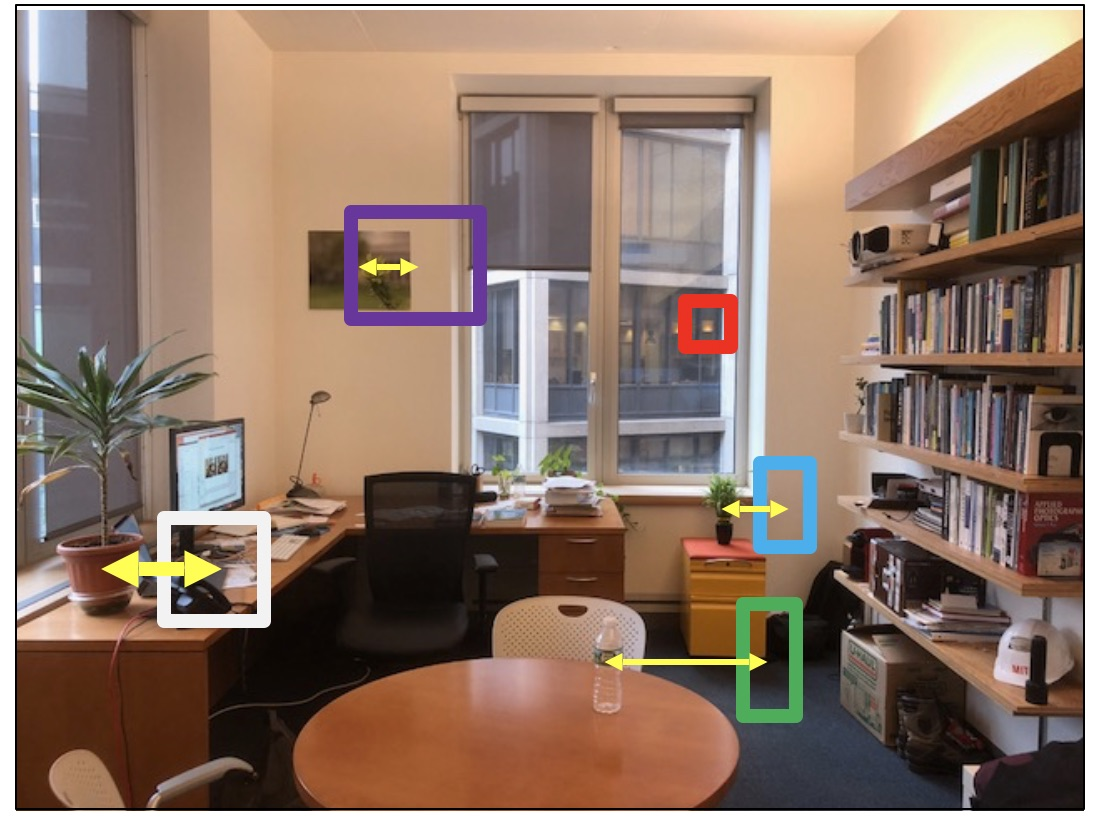
\includegraphics[width=0.475\linewidth]{figures/stereo/officeRight.jpg}}
    }
    \caption{Two cameras, displaced from each other laterally, photograph the same scene, resulting in images (a) and (b).  Colored rectangles show some identifiable features in image (a), and where those features appear in image (b).  Arrows show the corresponding displacements, which reveal depth through \eqn{\ref{eq:depthFromDisparity}}.}
    \label{fig:stereomatch}
\end{figure}



A naive algorithm for finding the disparity of any pixel in the left image is to search for a pixel of the same intensity  in the corresponding row of the right image.  \Fig{\ref{fig:stereolamp}}, from \cite{Hosni2013}, shows why that naive algorithm won't work and why this problem is hard. \Fig{\ref{fig:stereolamp}}{a} shows the intensities of one row of the right-eye image of a stereo pair. The squared difference of the intensity differences from offset versions of the same row in the rectified left-eye image of the stereo pair is shown in \fig{\ref{fig:stereolamp}}{b}, for a range of disparity offsets, plotted vertically, in a configuration known as the {\bf disparity space image} \cite{Scharstein2002}.  The disparity corresponding to the minimum squared error matches are plotted in red.  Note the disparities of the best pixel intensity matches show much more disparity variations than would result from the smooth surfaces depicted in the image; the local intensity matches don't reliably indicate the disparity.  Many effects lead to that unreliability, including: lack of texture in the image, which leads to noisy matches among the many nearly identical pixels; image intensity noise; specularities in the image which change location from one camera view to another; and scene points appearing in one image but not another due to occlusion. \Fig{\ref{fig:stereolamp}}{d} shows an effective approach to remove the matching noise:  blurring the disparity space image using an edge-preserving filter \cite{Hosni2013}.  The best-matched disparities are plotted in red, and compare well with the ground truth disparities (\fig{\ref{fig:stereolamp}}[f]), as labeled in the dataset \cite{Scharstein2002}.


\begin{figure}[t]
    \centerline{
        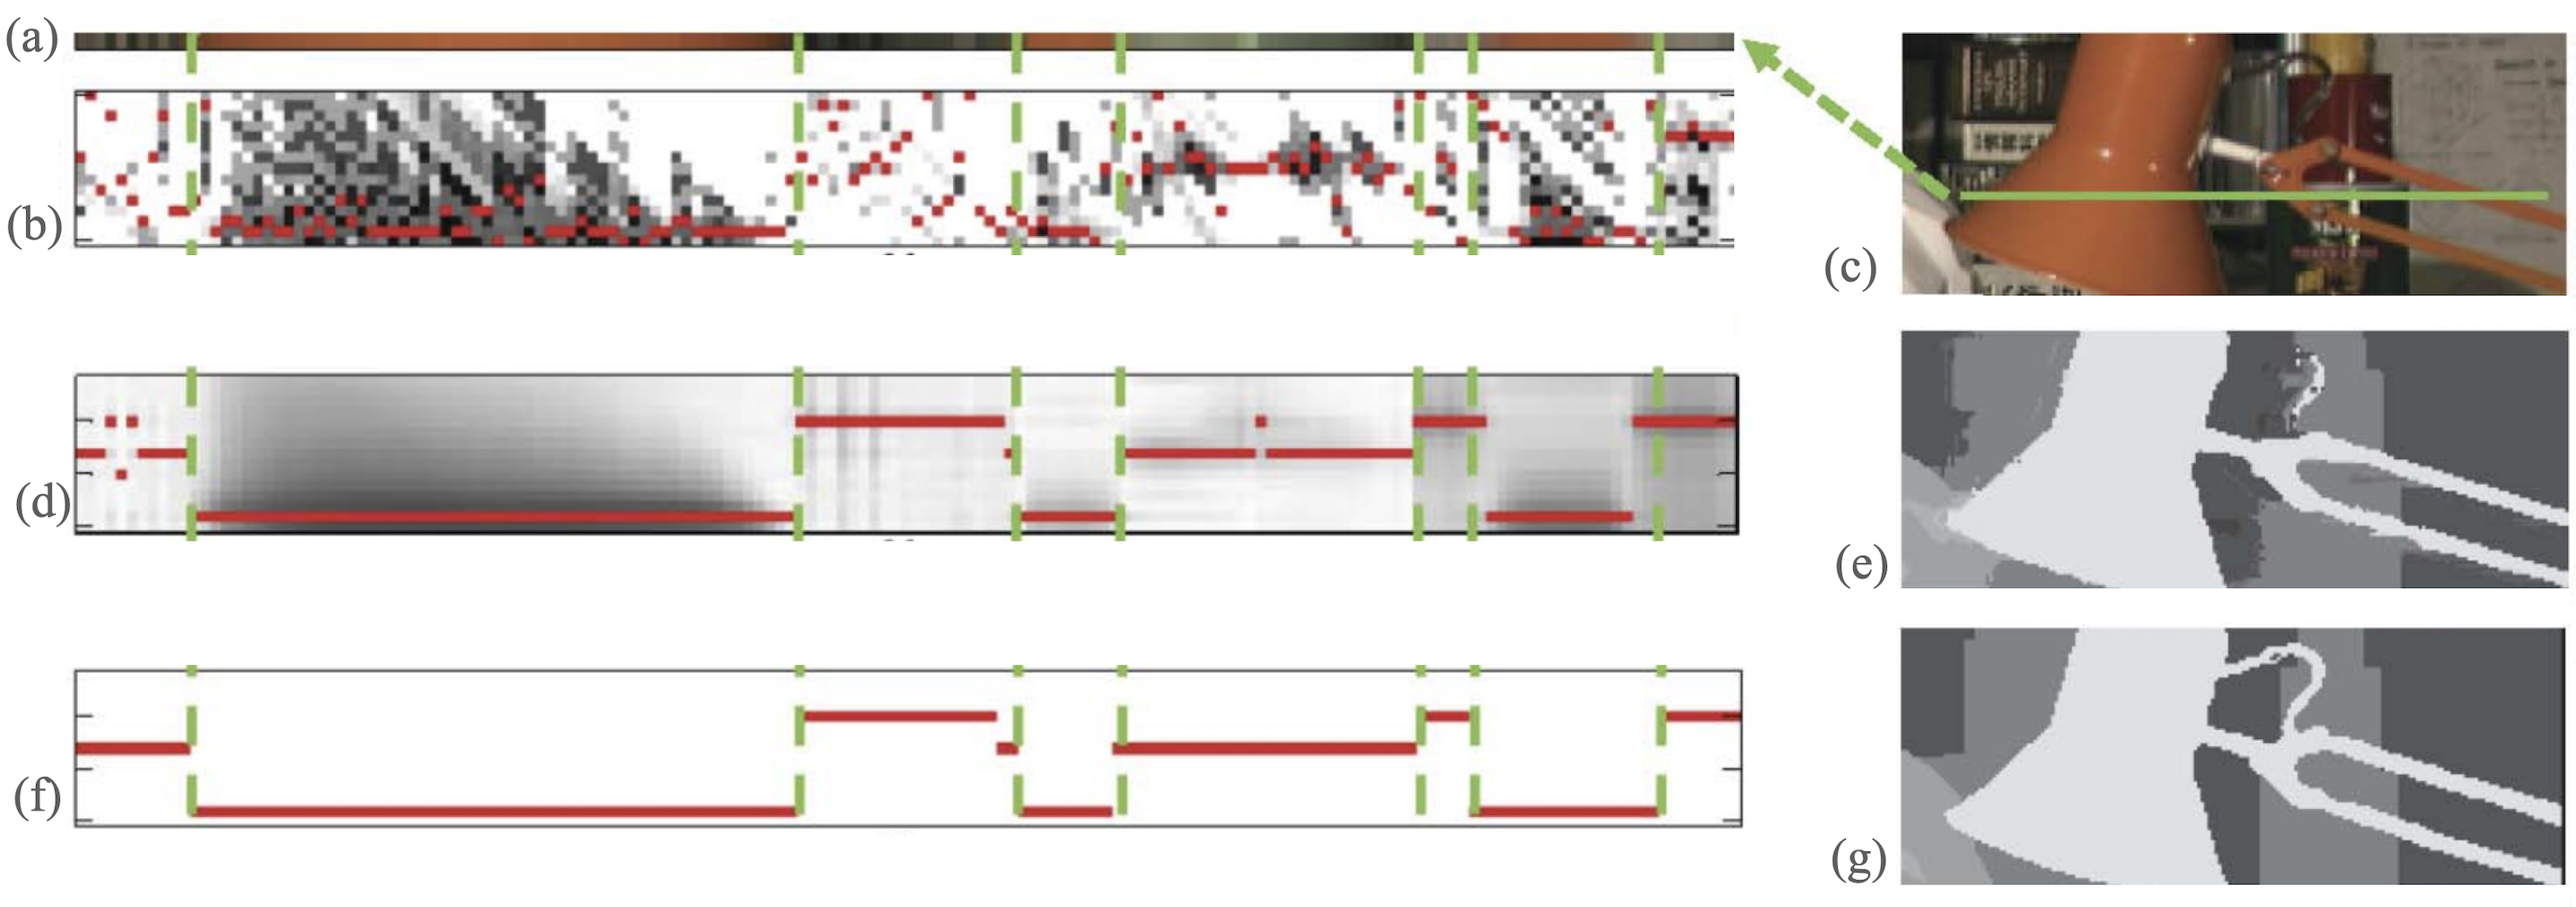
\includegraphics[width=1\linewidth]{figures/stereo/stereolamp.jpg}}
    \caption{Issues with intensity-based stereo matching.
        %(a) One line of one image, (c), of stereo pair. (b) Intensity matching error for different disparities, plotted vertically, as a function of horizontal position.  Red shows disparities of best intensity match. (d) Smoothed matching errors, with best matches shown in red, and resulting depth image, (e).  (f) Ground truth matches and depth (g).  
        Dataset from \cite{Scharstein2002}. Figure modified from \cite{Hosni2013}.}
    \label{fig:stereolamp}
    %\vspace{-1.2in}
\end{figure}

The task of finding disparity at each point is often broken into two parts:  (1) finding features, and matching the features across images, and (2) interpolating between, or adjusting, the feature matches to obtain a reliable disparity estimate everywhere.
These two steps are often called matching and filtering, because the interpolation can be performed using filtering methods.

We will describe next a classical method to find key points and extract image descriptors to find image correspondences. In \chap{\ref{chapter:3D_multiview}} we will describe other learning-based approaches.

\subsubsection{Finding image features}
\label{sec:finding_image_features}
%~\\

Good image features are positions in the image that are easy to localize, given only the image intensities. The {\bf Harris corner detector} \cite{Harris88}
\index{Harris corner detector}
identifies image points that are easy to localize by evaluating how the sum of squared intensity differences over an image patch change under a small translation of the image. If the squared intensity changes quickly with patch translation in every direction, then the region contains a good image feature.

To derive the equation of the Harris corner detector we will compute image derivatives. Therefore, we will write an image as a continuous function on $x$ and $y$. The compute the final quantities in practice we will approximate the derivatives using their discrete approximations as discussed in \chap{\ref{chapter:image_derivatives}}. Let the input image be $\img (x,y)$, and let the small translation be $\Delta x$ in $x$ and $\Delta y$ in $y$.  Then, the squared intensity difference, $E(\Delta x, \Delta y)$, induced by that small translation, summed over a small image patch, $P$, is
\begin{equation}
    E(\Delta x, \Delta y) = \sum_{(x, y) \in P}
    \left(
    \img(x,y) - \img(x + \Delta x, y + \Delta y)
    \right)^2
    \label{eq:harris}
\end{equation}

We expand $\img (x + \Delta x, y + \Delta y)$ about $\img (x, y)$ in a Taylor series:
\begin{equation}
    \img (x + \Delta x, y + \Delta y) \approx
    \img (x, y) + \frac{\partial \img}{\partial x} \Delta x
    + \frac{\partial \img}{\partial y} \Delta y
\end{equation}
Substituting the above into \eqn{\ref{eq:harris}} and writing the result in matrix form yields
\begin{equation}
    E(\Delta x, \Delta y) \approx
    \left[
        %\begin{array}{c c}
        \Delta x ~~ \Delta y
        %\end{array}
        \right]
    \mathbf{M}
    \left[ \begin{array}{c}
            \Delta x \\
            \Delta y
        \end{array}
        \right]
\end{equation}
where
\begin{equation}
    \mathbf{M} = \sum_{(n, m) \in P}
    \begin{bmatrix}
        (\frac{\partial \img}{\partial x})^2 &
        \frac{\partial \img}{\partial x}
        \frac{\partial \img}{\partial y}                                            \\
        \frac{\partial \img}{\partial x}
        \frac{\partial \img}{\partial y}
                                             & (\frac{\partial \img}{\partial y})^2
    \end{bmatrix}
\end{equation}

The smallest eigenvalue, $\lambda_{\mbox{min}}$ of the matrix, $\mathbf{M}$, indicates the smallest possible change of image intensities under translation of the patch in any direction.  Thus, to detect good corners, one can identify all points for which $\lambda_{\mbox{min}} > \lambda_c$, for some threshold $\lambda_c$.
The Harris corner detector has been widely used for identifying features to match across images, although they were later supplanted by the scale-invariant feature transform (SIFT) \cite{Lowe04},
\index{SIFT}
based on maxima over a scale of Laplacian filter outputs.  Figures \ref{fig:stereopoints}(a and b) show the result of the Harris feature detector to the images of \fig{\ref{fig:stereomatch}}.


\begin{figure}[h]
    \centerline{
        \sublabel{a}{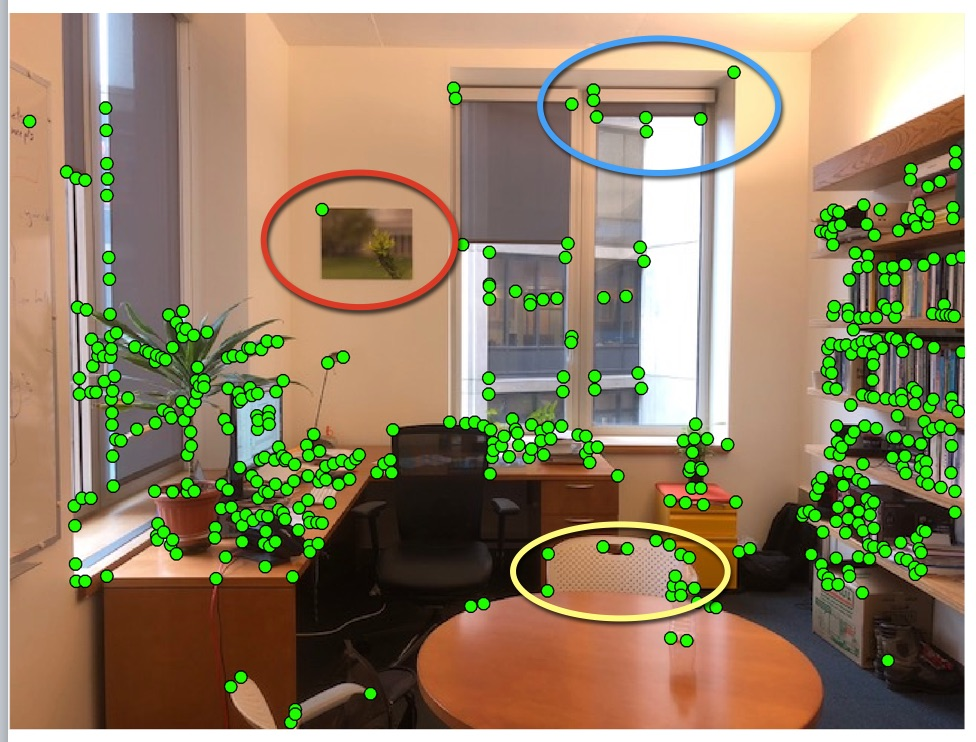
\includegraphics[width=0.31\linewidth]{figures/stereo/pointsLeft.jpg}}
        \sublabel{b}{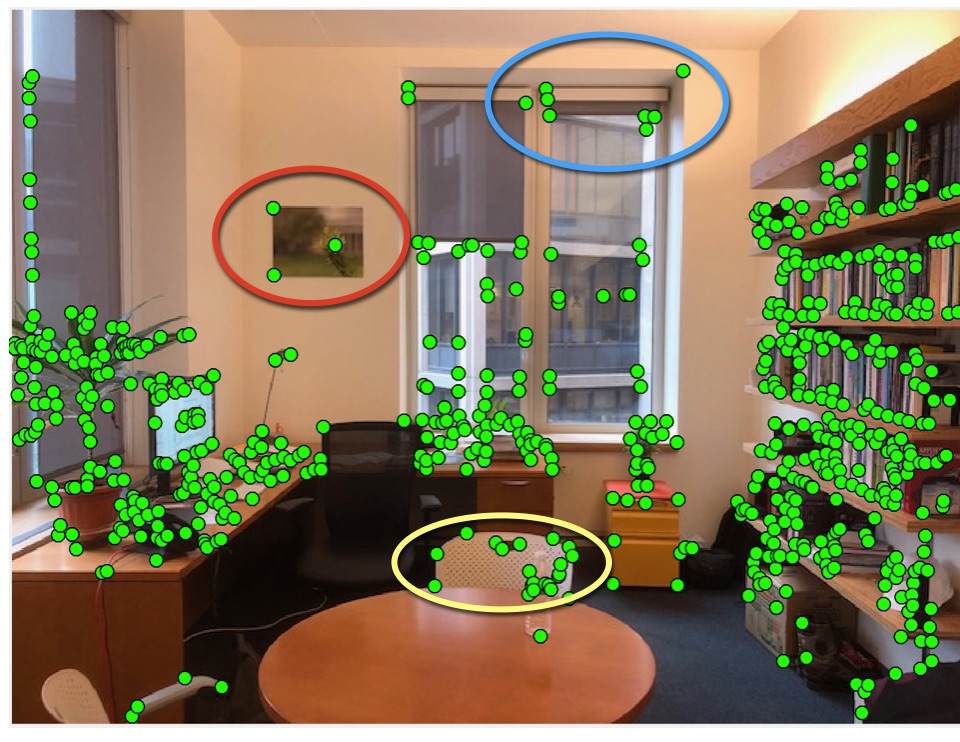
\includegraphics[width=0.31\linewidth]{figures/stereo/pointsRight.jpg}}
        \sublabel{c}{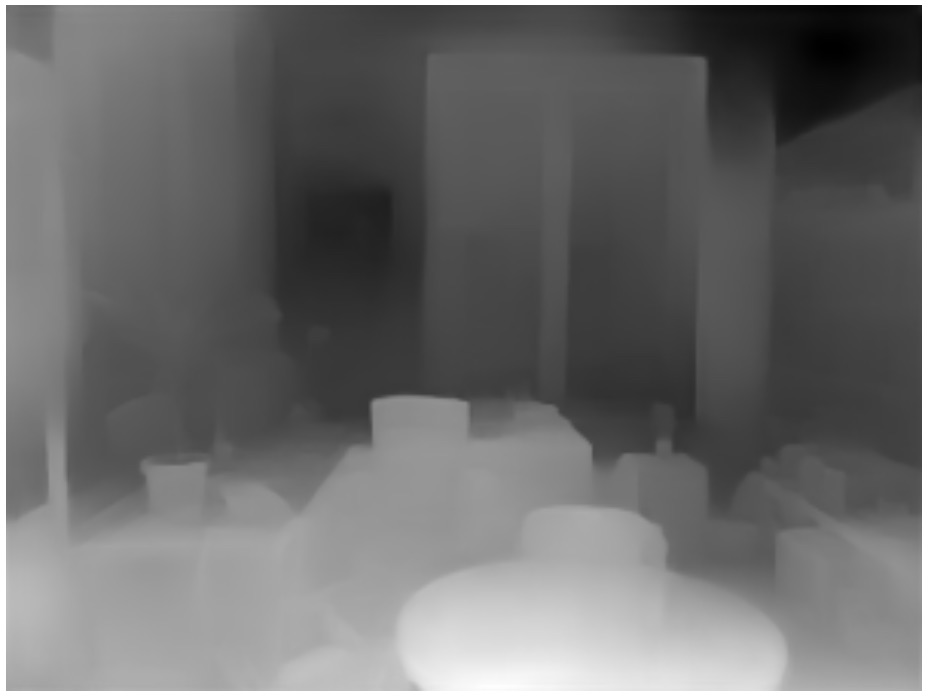
\includegraphics[width=0.31\linewidth]{figures/stereo/officeDepth.jpg}}
    }
    \caption{The feature-based stereo approach, illustrated for the stereo pair of \fig{\ref{fig:stereomatch}}. (a and b) Feature points. (c) Depth image.
        %Feature points are found, independently, in each of the stereo pair images (a) and (b).  Detected Harris feature points \cite{Harris88} are shown as green dots. It is especially visible within the marked ellipses that not the same set of feature points is marked in each image.  (c) shows a depth image resulting from a matched and interpolated set of feature points.
    }
    \label{fig:stereopoints}
\end{figure}
%\vspace{-1.35in}

Figures \ref{fig:stereopoints}(a and b) reveal the challenges of the feature matching task:  (1) not every feature is marked across both images, and (2) we need to decide which pairs of image features go together.  Feature points are found, independently, in each of the stereo pair images (figures \ref{fig:stereopoints}[a and b]).  Detected Harris feature points \cite{Harris88} are shown as green dots. It is especially visible within the marked ellipses that not the same set of feature points is marked in each image.  \Fig{\ref{fig:stereopoints}}{c} shows a depth image resulting from a matched and interpolated set of feature points.

\subsubsection{Local image descriptors}
%~\\
Matching corresponding image features require a local description of the image region to allow matching like regions across two images.  SIFT  \cite{Lowe04} uses histograms of oriented filter responses to create an image descriptor that is sensitive to local image structure, but that is insensitive to minor changes in lighting or location which may occur across the two images of a stereo pair.

\Fig{\ref{fig:SIFT}} shows a sketch of the use of oriented edges and SIFT descriptors in image analysis. The top row of \fig{\ref{fig:SIFT}}{a} shows two images of a hand under different lighting conditions. Despite that both images look quite different in a pixel intensity representation, they look quite similar in a local orientation, depicted in the bottom row by line segment directions.  SIFT image descriptors \cite{Lowe04} exploit that observation.  Taking histograms (\fig{\ref{fig:SIFT}}[b]) of local orientation over local spatial regions further allow for image descriptors to be robust to small image translations \cite{Freeman98c,Lowe04}.

\begin{figure}[h!]
    \centerline{
        \sublabel{a}{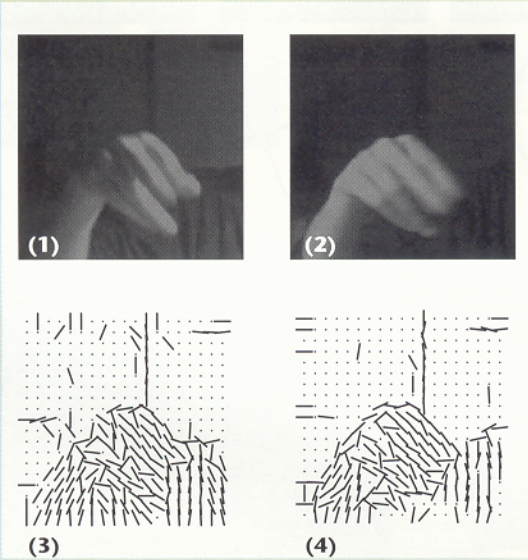
\includegraphics[width=0.4\linewidth]{figures/stereo/hands.jpg}}
        \sublabel{b}{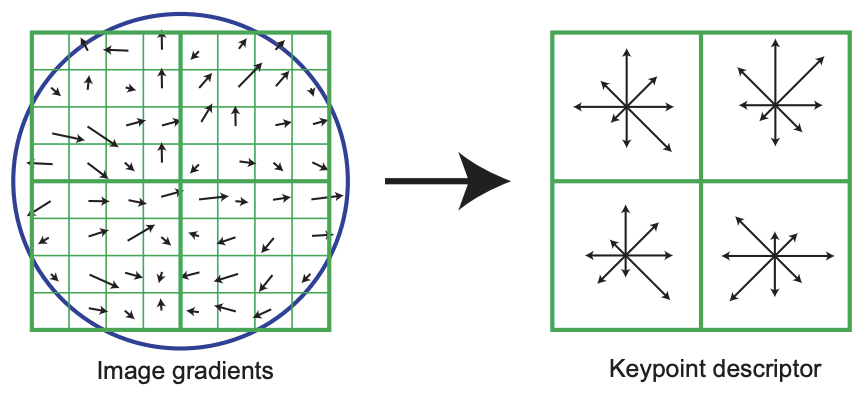
\includegraphics[width=0.5\linewidth]{figures/stereo/SIFT.jpg}}
    }
    \caption{Orientation-based image descriptors.  (a) Oriented features. Reprinted from \cite{Freeman98c}.  (b) SIFT image descriptors \cite{Lowe04}.}
    \label{fig:SIFT}
\end{figure}

\subsubsection{Interpolation between feature matches}
%~\\
Methods to interpolate depth between the depths of matched points include probabilistic methods such as belief propagation, discussed in
\chap{\ref{chapter:probabilistic_graphical_models}}.
Under assumptions about the local spatial relationships between depth values, optimal shapes can be inferred provided the spatial structure over which inference is performed is a chain or a tree.  Note that \cite{Hirschmuller2007} uses a related inference algorithm, dynamic programming, which has the same constraints on spatial structure for exact inference.  Hirschmuller's algorithm, called semiglobal matching (SGM), applies the one-dimensional processing over many different orientations to approximate a global solution to the stereo shape inference problem.


\subsection{Constraints for Arbitrary Cameras}

Until now we have considered only the case where the two cameras are parallel, but in general the two images will be produced by cameras that can have arbitrary orientations. Note that disparity of the smokestacks in \fig{\ref{fig:titanic}}{a} increases with depth, rather than decreasing as described by \eqn{\ref{eq:depthFromDisparity}}.  That is because the cameras that took the stereo pair were not in the same orientation, related only by a translation.

%In closing, we   After rectification, the stereo image pair of Fig.~\ref{fig:titanic}~(a) would obey the depth-disparity relation of Eq.~(\ref{eq:depthFromDisparity}).




% Useful: https://en.wikipedia.org/wiki/Essential_matrix

Let's assume we have two calibrated cameras: we know the intrinsic and extrinsic parameters for both. They are related by a generic translation, $\mathbf{T}$, and a rotation, $\mathbf{R}$, such that their optical axis are not parallel. Let's now consider that we see one point in the image produced by camera 1 and we want to identify where is the corresponding point in the image from camera 2. The following sketch (\fig{\ref{fig:epipolar_1}}) shows the setting of the problem we are trying to solve.

\begin{figure}[h!]
    \centerline{
        \includegraphics[width=0.7\linewidth]{figures/3d_scene_understanding/epipolar_1.eps}
    }
    \caption{How can we identify the specific point $\mathbf{p}_2$ on camera 2 that represents the projection of the same 3D point as $\mathbf{p}_1$ on camera 1?}
    \label{fig:epipolar_1}
\end{figure}

Are there any geometric constraints that can help us to identify candidate matches? We know that the observed point in camera 1, $\mathbf{p}_1$, corresponds to a 3D point that lies within the ray that connects the camera 1 origin and $\mathbf{p}_1$ (shown in red in \fig{\ref{fig:epipolar_3}}):

\begin{figure}[h!]
    \centerline{
        \includegraphics[width=0.7\linewidth]{figures/3d_scene_understanding/epipolar_3.eps}
    }
    \caption{The point $\mathbf{p}_1$ corresponds to a 3D point that lies within the ray that connects the camera 1 origin and $\mathbf{p}_1$. The point $\mathbf{p}_2$ is constrained to be within the projection of that line on camera 2.}
    \label{fig:epipolar_3}
\end{figure}

Therefore, $\mathbf{p}_2$ is constrained to be within the line that results of projecting the ray into camera 2. Remember that a line in 3D projects into a line in 2D. There are two points that are of particular interest in the line projected into camera 2. The first point is the projection of the camera center of camera 1 into the camera plane 2 (the point could lay outside the camera view but in this example it happens to be visible). The second point is the projection of $\mathbf{p}_1$ itself into camera 2. As we know all the intrinsic and extrinsic camera parameters, those two points should be easy to calculate. And these two points will define the equation of the line (there are many other ways to think about this problem).



%\subsubsection{Stereo geometry}

The following figure shows the geometry of a stereo pair. Given a 3D point, $\mathbf{P}$, in the world, we define the following objects:
\begin{itemize}
    \item The {\bf epipolar plane}\index{Epipolar plane} is the plane that contains the two camera origins and a 3D point, $\mathbf{P}$.

    \item The {\bf epipolar lines}\index{Epipolar line} are the intersection between the epipolar plane and the camera planes. When the point $\mathbf{P}$ moves in space, the epipolar plane and epipolar lines change.

    \item The {\bf epipoles}\index{Epipole} are the intersection points between the line that connects both camera origins and the camera planes.  The epipoles' location does not depend on the point $\mathbf{P}$. Therefore, all the epipolar lines intersect at the same epipoles.
\end{itemize}

\begin{figure}[h!]
    \centerline{
        \includegraphics[width=0.8\linewidth]{figures/3d_scene_understanding/epipolar_geometry.eps}
    }
    \caption{Geometry of a stereo pair and terminology. The figure shows the epipolar plane, epipolar lines, and epipoles ($e_1$ and $e_2$), for a given point $\mathbf{P}$. As we move the point $\mathbf{P}$, only the epipoles remain constant.}
    \label{fig:epipolar_geometry_terminology}
\end{figure}

In the example shown in \fig{\ref{fig:epipolar_geometry_terminology}}, as both cameras are only rotated along their vertical axis and there is no vertical displacement between them, the epipoles are contained in the $x$ axes of both camera coordinate systems.
The epipolar line in camera 2, corresponds to the projection of the line $O_1 P$ into the camera plane. Therefore, given the image point $\mathbf{p}_1$, we know that the match should be somewhere along the epipolar line.

The epipolar line in camera 2 that corresponds to $\mathbf{p}_1$ is uniquely defined by the camera geometries and the location of image point $\mathbf{p}_1$. So, when looking for matches of a point in one camera, we only need to look along the corresponding epipolar line in the other camera. The same applies for finding matches in camera 1 given a point in camera 2.

In the next section we will see how to find the epipolar lines  mathematically.


\subsection{The Essential and Fundamental Matrices}

We will follow here the derivation that was proposed by Longuet-Higgins, in 1981 \cite{Longuet-Higgens1981}.
%https://cseweb.ucsd.edu/classes/fa01/cse291/hclh/SceneReconstruction.pdf
Let's consider a 3D point, $\mathbf{P}$, viewed by both cameras. The coordinates of this 3D point $\mathbf{P}$ are $\mathbf{P}_1 = [X_1,Y_1,Z_1]^\transpose$ when expressed in the coordinates system of camera 1, and $\mathbf{P}_2= [X_2,Y_2,Z_2]^\transpose$ when expressed in the coordinates system of camera 2. Both systems are related by (using heterogeneous coordinates):
\begin{equation}
    \mathbf{P}_2 = \mathbf{R} \mathbf{P}_1 + \mathbf{T}
    \label{eq:relation1}
\end{equation}

The 3D point $\mathbf{P}_1$ projects into the camera 1 at the coordinates
$\mathbf{p}_1 = f \mathbf{P}_1 /Z_1$ where $\mathbf{p}_1$ is expressed also in 3D coordinates $\mathbf{p}_1 = [f X_1/Z_1, f Y_1/Z_1, f]^\transpose$. Without losing generality we will assume $f=1$.

Taking the cross product of both sides of \eqn{\ref{eq:relation1}} with $\mathbf{T}$ we get:
\begin{equation}
    \mathbf{T} \times \mathbf{P}_2 = \mathbf{T} \times \mathbf{R} \mathbf{P}_1
    \label{eq:relation2}
\end{equation}
as $\mathbf{T} \times \mathbf{T} = 0$. And now, taking the dot product of both sides of \eqn{\ref{eq:relation2}} with $\mathbf{P}_2$:
\begin{equation}
    \mathbf{P}_2^\transpose \mathbf{T} \times \mathbf{P}_2 = \mathbf{P}_2^\transpose \mathbf{T} \times \mathbf{R} \mathbf{P}_1
\end{equation}

The left side is zero because $\mathbf{T} \times \mathbf{P}_2$ results in a vector that is orthogonal to both $\mathbf{T}$ and $\mathbf{P}_2$, and the dot product with $\mathbf{P}_2$ is zero (dot product of two orthogonal vectors is zero). Therefore, $\mathbf{P}_1$ and $\mathbf{P}_2$ satisfy the following relationship:
\begin{equation}
    \mathbf{P}_2^\transpose \left( \mathbf{T} \times \mathbf{R} \right) \mathbf{P}_1 = 0
\end{equation}


\marginnote{The cross product of two vectors $\mathbf{a} \times \mathbf{b}$ can be written in matrix form as:
    \begin{equation*}
        \mathbf{a} \times \mathbf{b} =
        \mathbf{a}_{\times} \mathbf{b}
    \end{equation*}
    The special matrix $\mathbf{a}_{\times}$ is defined as:
    \begin{equation*}
        \mathbf{a}_{\times} =
        \begin{bmatrix}
            0    & -a_3 & a_2  \\
            a_3  & 0    & -a_1 \\
            -a_2 & a_1  & 0    \\
        \end{bmatrix}
    \end{equation*}
    This matrix $\mathbf{a}_{\times}$ is rank 2. In addition, it is a skew-symmetric matrix (i.e., $\mathbf{a}_{\times} = -\mathbf{a}_{\times}^\transpose$). It has two identical singular values and the third one is zero.
}

The matrix $\mathbf{E}$ is called the {\bf essential matrix} and it corresponds to: \index{Essential matrix}
\begin{equation}
    \mathbf{E} =  \mathbf{T} \times \mathbf{R} = \mathbf{T}_{\times} \mathbf{R}
\end{equation}
This results in the relationship:
\begin{equation}
    \mathbf{P}_2^\transpose \mathbf{E} \mathbf{P}_1 = 0
    \label{eq:relation3}
\end{equation}

If we divide \eqn{\ref{eq:relation3}} by $Z_1 Z_2$ we will obtain the same relationship but relating the image coordinates:

\begin{equation}
    \mathbf{p}_2^\transpose \mathbf{E} \mathbf{p}_1 = 0
    \label{eq:relation4}
\end{equation}
This equation relates the coordinates of the two projections of a 3D point into two cameras. If we fix the coordinates from one of the cameras, the equation reduces to the equation of a line for the coordinates of the other camera, which is consistent with the geometric reasoning that we made before.

The essential matrix is a 3 $\times$ 3 matrix with some special properties:
\begin{itemize}
    \item $\mathbf{E}$ has five degrees of freedom instead of nine. To see this, let's count degrees of freedom: the rotation and translation have three degrees of freedom each, this gives six; then, one degree is lost in \eqn{\ref{eq:relation4}} as a global scaling of the matrix does not change the result. This results in five degrees of freedom.

    \item The essential matrix has rank 2. This is because $\mathbf{E}$ is the product of a rank 2 matrix, $\mathbf{T}_{\times}$, and a rank 3 matrix, $\mathbf{R}$.

    \item The essential matrix has two identical singular values and the third one is zero. This is because $\mathbf{E}$ is the product of $\mathbf{T}_{\times}$, which has two identical singular values, and the rotation matrix $\mathbf{R}$ that does not change the singular values.
\end{itemize}
As a consequence, not all 3 $\times$ 3 matrices correspond to an essential matrix which is important when trying to estimate $\mathbf{E}$.


\subsubsection{The fundamental matrix} \index{Fundamental matrix}
%~\\
We have been using camera coordinates, $\mathbf{p}$. If we want to use image coordinates, in homogeneous coordinates, $\mathbf{c}=[n,m,1]^\transpose$, we need to also incorporate the intrinsic camera parameters (which will also incorporate pixel size and change of origin). Incorporating the transformation from camera coordinates, $\mathbf{p}$, to image coordinates, $\mathbf{c}$, the equation relating image coordinates in both cameras has the same algebraic form as in \eqn{\ref{eq:relation4}}:

\begin{equation}
    \mathbf{c}_2^\transpose \mathbf{F} \mathbf{c}_1 = 0
\end{equation}
where $\mathbf{F}$ is the {\bf fundamental matrix}.

The fundamental and essential matrices are related via the intrisic camera matrix, namely:
\begin{equation}
    \mathbf{F} = \mathbf{K}^{-\transpose} \mathbf{E} \mathbf{K}^{\transpose}
\end{equation}

The fundamental matrix has rank 2 (like the essential matrix) and 7 degrees of freedom (out of the 9 degrees of freedom, one is lost due to the scale ambiguity and another is lost because the determinant has to be zero).

\subsubsection{Estimation of the essential/fundamental matrix}
%~\\
Given a set of matches between the two views we can estimate either the essential or the fundamental matrix by writing a linear set of equations. Any two matching points will satisfy $\mathbf{p}_2^\transpose \mathbf{E} \mathbf{p}_1 = 0$ and we can use this a linear set of equations for the coefficients of $\mathbf{E}$. However, the matrix $\mathbf{E}$ has a very special structure that allows more efficient and robust methods to estimate the coefficients. The same applies for the fundamental matrix.

As both matrices are rank 2, the minimization the linear set of equations can be done using a constrained minimization or directly optimizing a rank 2 matrix. You can also delete the third singular value $\mathbf{F}$, and, for $\mathbf{E}$, you can delete the third singular value and set the first and second singular values to be equal.

Once $\mathbf{E}$ is estimated, it can be decomposed to recover the translation (skew-symmetric matrix) and rotation (orthonormal matrix) between the two cameras using the singular value decomposition methods.

\subsubsection{Finding the epipoles}
%~\\
As the epipoles, $\mathbf{e}_1$ and $\mathbf{e}_2$, belong to the epipolar lines, they satisfy
\begin{equation}
    \mathbf{p}_2^\transpose \mathbf{E} \mathbf{e}_1 = 0
\end{equation}\begin{equation}
    \mathbf{e}_2^\transpose \mathbf{E} \mathbf{p}_1 = 0
\end{equation}
and, as the epipoles are the intersection of all the epipolar lines, both relationships shown previously have to be true for any points $\mathbf{p}_1$ and $\mathbf{p}_2$. Therefore,
\begin{equation}
    \mathbf{E} \mathbf{e}_1 = 0
\end{equation}\begin{equation}
    \mathbf{e}_2^\transpose \mathbf{E} = 0
\end{equation}
As the matrix $\mathbf{E}$ is likely to be noisy, we can compute the epipoles as the eigenvectors with the smallest eigenvalues of $\mathbf{E}$ and $\mathbf{E}^\transpose$.


\subsubsection{Epipolar lines: The game}
%~\\
In order to build an intuition of how epipolar lines work we propose to play a game.
\Fig{\ref{fig:epipolarlinesgame}} shows a set of camera pairs and a set of epipolar lines. Can you guess what camera pair goes with what set of epipolar lines? \footnote{Answer for the game in \fig{\ref{fig:epipolarlinesgame}}: A-2, B-5, C-4, D-6, E-3, F-1.}


\begin{figure}[t]
    \centerline{
        \includegraphics[width=1\linewidth]{figures/3d_scene_understanding/epipolar_game_play.eps}
    }
    \caption{Epipolar game. The figure shows six camera pair arrangements, and six sets of epipolar lines. Can you identify which camera pairs correspond to each set of epipolar lines?}
    \label{fig:epipolarlinesgame}
\end{figure}

To solve the game, visualize mentally the cameras and think about how rays from the origin of one camera will be seen from the other camera. The epipole corresponds to the location where one camera sees the origin of the other camera.

Observe that most of the sets of epipolar lines shown in the figure are symmetric across the two cameras, but it is not always true. What conditions are needed to have symmetric epipolar lines across both cameras? What camera arrangements will break the symmetry? If you were to place two cameras in random locations, do you expect to see symmetric epipolar lines?

It is also useful to use the equations defining the epipolar lines and deduce the equations for the epipolar lines for some of the special cases shown in \fig{\ref{fig:epipolarlinesgame}}.

\marginnote{When building systems, it is crucial to visualize intermediate results in order to find bugs in code. This requires knowing what the results should look like. The game from \fig{\ref{fig:epipolarlinesgame}} helps building that understanding.}[-1in]

\subsection{Image Rectification}

%Another application of the homography transformations described in Chapt. YY is a stereo pre-processing step called {\bf image rectification}.  

As described previously, one only needs to search along epipolar lines to find matching points in the second image.  If the sensor planes of each camera are coplanar, and if the pixel rows are colinear across the two cameras, then the epipolar lines will be along image scanlines, simplifying the stereo search.


Using the homography transformations (\chap{\ref{chapter:homography}}), we can warp observed stereo camera images taken under general conditions to synthesize the images that would have been recorded had the cameras been aligned to yield epipolar lines along scan rows.


Many configurations of the two cameras satisfy the desired image rectification constraints \cite{Zhang2003}: (1) that epipolar lines are along image scanlines, and (2) that matching points are within the same rows in each camera image.  One procedure that will satisfy those constraints is as follows \cite{wikiRectification2021}.  First, rotate each camera to be parallel with each other and with optical axes perpendicular to the line joining the two camera centers.  Second, rotate each of the cameras about its optical axis to align the rows of each camera with those of the other.  Third, uniformly scale one camera's image to be the same size as to the other, if necessary.  The resulting image pair will thus satisfy the two requirements above for image rectification. Image rectification uses image warping with bilinear (or other) interpolation as described in \sect{\ref{sec:bilinearinterpolation}}.

Other algorithms are optimized to minimize image distortions \cite{Zhang2003} and may give better performance for stereo algorithms.  We assume camera calibrations are known, but other rectification algorithms can use weaker conditions, such as knowing the fundamental matrix \cite{Hartley2004,Pollefeys99}. Many software packages provide image rectification code \cite{Zhang99}.



%\subsection{Active stereo}

%Brief mention about using structured light using projectors. 

%stereo / rgb-d




\section{Learning-Based Methods}

As is the case for most other vision tasks, neural network approaches now dominate stereo methods.  The two stages of a stereo algorithm, matching and filtering, can be implemented separately by neural networks \cite{Zbontar2015}, or together in a single, end-to-end optimization (\cite{Zhang2019GANet,Chang2018,Mayer2016,Kendall2017}.

\subsection{Output Representation}

One important question is how  we want to represent the output. We are ultimately interested in estimating the 3D structure of the scene. We can estimate the disparity or the depth. Disparity might be easier to estimate as it is independent of the camera parameters. It is also easier to model noise, as we can assume that noise is independent of disparity. However, when using depth, estimation error will be larger for distant points.

Another interesting property of disparity is that for flat surfaces, the second-order derivative along any spatial direction, $\mathbf{x}$, is zero:
\begin{equation}
    \frac{\partial^2 d}{\partial \mathbf{x}^2}  = 0.
\end{equation}
This equality does not hold for depth. This property allows introducing a simple regularization term that favors planarity.

To translate the returned disparity for a given pixel $d\left[n,m \right]$ into depth values $z\left[n,m \right]$, we need to invert the disparity, that is

\begin{align}
    z \left[n,m \right] = \frac{1}{ d \left[n,m \right] }
\end{align}
Now we need to recover the world coordinates for every pixel.
Assuming a pinhole camera and using the depth, $z \left[n,m \right]$, and the intrinsic camera parameters, $\mathbf{K}$, we obtain the 3D coordinates for a pixel with image coordinates $[n,m]$ in the camera reference frame as
\begin{align}
    \begin{bmatrix}
        X \\
        Y \\
        Z
    \end{bmatrix}
    = z\left[n,m \right] \times \mathbf{K}^{-1} \times
    \begin{bmatrix}
        n \\
        m \\
        1
    \end{bmatrix}
\end{align}
Note that $\mathbf{K}$ are the intrinsic camera parameters for the reference image.

\subsection{Two-Stage Networks}
Given two images, $\mathbf{v}_1$ and $\mathbf{v}_2$, the disparity at each location can be computed by a function, that is:
\begin{equation}
    \hat{\mathbf{d}} = f_{\theta}(\mathbf{v}_1, \mathbf{v}_2)
\end{equation}

The objective is that the estimated disparities, $\hat{\mathbf{d}}$, should be close to ground truth disparities, $\mathbf{d}$. One example of training set are the KITTI dataset \cite{Geiger2013} and the scene flow dataset \cite{Mayer2016}, which contain ground truth disparities  from calibrated stereo cameras. One typical loss is:
\begin{equation}
    J(\theta) = \sum_t \left| \mathbf{d} - f_{\theta} (\mathbf{v}_1, \mathbf{v}_2) \right|^2
\end{equation}
This is optimized by gradient descent as usual.

%https://lmb.informatik.uni-freiburg.de/Publications/2016/MIFDB16/paper-MIFDB16.pdf

When matching and filtering are implemented separately, one common formulation is to use one neural network to extract features from both images, $g(\mathbf{i}_1)$ and $g(\mathbf{i}_2)$, and one neural network to compute the matching cost and estimate the disparities at every pixel.
\begin{equation}
    f(\mathbf{v}_1, \mathbf{v}_2) = c \left( g(\mathbf{v}_1), g(\mathbf{v}_2) \right)
\end{equation}


A common approach, depicted in block diagram form in \fig{\ref{fig:stereoblock}}, is the following:
\begin{itemize}
    \item Rectify the stereo pair so that scanlines in each image depict the same points in the world.
    \item Extract features from each image, using a pair of networks with shared weights.
    \item Form a 3D cost volume indicating the local visual evidence of a match between the two images for each possible pixel position and each possible stereo disparity.  (This 3D cost volume can be referenced to the $H$ and $V$ positions of one of the input images.)
    \item Train and apply a 3D convolutional neural net (CNN) to aggregate (process) the costs over the 3D cost volume in order to estimate a single, best disparity estimate for each pixel position.  This performs the function of the regularization step of nonneural-network approaches, such as SGM \cite{Hirschmuller2007}, but the performance is better for the neural network approaches.
\end{itemize}


\begin{figure}[t]
    \centerline{
        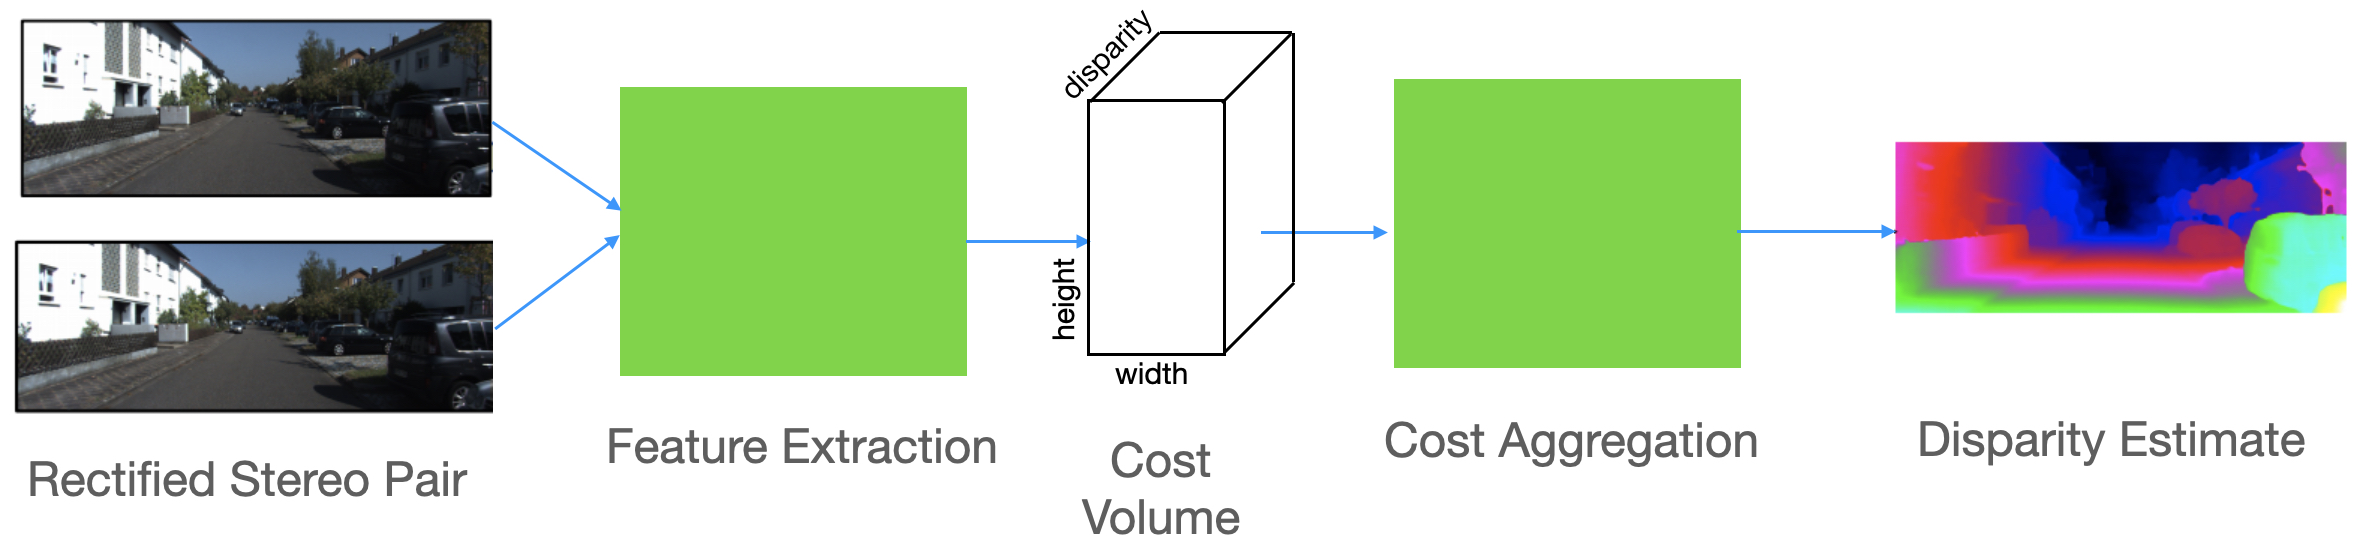
\includegraphics[width=1\linewidth]{figures/stereo/stereocnn.jpg}
    }
    \caption{Block diagram of CNN stereo processing, abstracted from the block diagrams of \cite{Chang2018,Zhang2019GANet,Kendall2017}.}
    \label{fig:stereoblock}
\end{figure}

The performance of methods following the block diagram of \fig{\ref{fig:stereoblock}} surpassed that of methods with handcrafted features.  More recent work has addressed the problem of poor generalization to out-of-training-domain test examples \cite{zhang2019domaininvariant}.  Training and computing the 3D neural network to process the cost volume can be expensive in time and memory and recent work has obtained both speed and performance improvement through developing an iterative algorithm to avoid the 3D filtering \cite{Lipson2021}.


%define the output: disparity or world coordinates? does it estimate also camera parameters or requires calibration?


%similar to single view, can be applied to any setting.

%make use of both stereo and single view cues

%scale invariant loss

%architectures: they can take as input rectified views from a calibrated stereo pair, or uncalibrated cameras.

%estimating 3D and camera parameters



%\section{Multiview geometry}

%Structure from motion.

%Bundle adjustment.

%PnP

%\subsection{Neural radiant fields}




\section{Evaluation}

The Middlebury stereo web page \cite{Scharstein2002} provides a comprehensive comparison of many stereo algorithms, compared on a common dataset, with pointers to algorithm descriptions and code.  One can use the web page to evaluate the improvement of stereo reconstruction algorithms over time.  The advancement of the field over time is very impressive.


\section{Concluding Remarks}

Accurate depth estimation from stereo pairs remains an unsolved problem. The results are still not reliable. In order to get accurate depth estimates, most methods require many images and the use of multiview geometry methods to reconstruct the 3D scene.

Stereo matching is often also formulated as a problem of estimating the image motion between two views captured at different locations. In \chap{\ref{chapter:motion_estimation}} we will discuss motion estimation algorithms.

We have only provided a short introduction to stereo vision, for an in depth study of the geometry of stereo pairs the reader can consult specialized books such as \cite{Hartley2004} and \cite{Faugeras93}.

